\documentclass[11pt,a4paper]{article}

\usepackage[utf8]{inputenc}
\usepackage[T1]{fontenc}
\usepackage[spanish,es-noquoting,es-nodecimaldot,es-tabla]{babel}
\usepackage{amsmath,amssymb,amsthm}
\usepackage{graphicx}
\usepackage{booktabs}
\usepackage{placeins}
\usepackage{microtype}
\usepackage[margin=2.7cm]{geometry}
\usepackage{xcolor}
\usepackage[font=small,labelfont=bf,margin=0.3cm]{caption}
\usepackage[colorlinks=true,linkcolor=azulosc,citecolor=azulosc,urlcolor=azulosc]{hyperref}

\definecolor{azulosc}{HTML}{1F4E79}
\definecolor{grisclaro}{HTML}{F2F2F2}

\usepackage{tcolorbox}
\tcbuselibrary{skins,breakable}

\newtcolorbox{idea}[1][]{
  colback=grisclaro, colframe=azulosc, boxrule=0.6pt, arc=2pt,
  left=6pt, right=6pt, top=5pt, bottom=5pt, breakable, #1}

\newtcolorbox{aviso}[1][]{
  colback=white, colframe=black!45, boxrule=0.6pt, arc=2pt,
  left=6pt, right=6pt, top=5pt, bottom=5pt, breakable, #1}

\newtcolorbox{pregunta}[1][]{
  colback=white, colframe=azulosc, boxrule=0.9pt, arc=2pt,
  left=6pt, right=6pt, top=5pt, bottom=5pt, breakable, #1}

\newcommand{\dd}{\mathrm{d}}
\newcommand{\ee}{\mathrm{e}}
\newcommand{\ii}{\mathrm{i}}
\newcommand{\rp}{p_r}
\graphicspath{{figuras/}}

\title{\bfseries Phase mixing con dispersión en momento angular:\\
       una introducción computacional al sistema de Vlasov--Poisson\\
       esférico con distribución en $L$}
\author{Notas de trabajo sobre el código \texttt{VlasovPoisson\_PIC\_sp}}
\date{}
\begin{document}
\maketitle

\begin{abstract}
\noindent
Estas notas son la continuación, para una distribución de momentos angulares, de las
notas del código con momento angular fijo (\texttt{vlasov-poisson\_PIC},
\texttt{docs/introduccion/vlasov\_intro.tex}). Están escritas para quien empieza con el
tema: se repasa la mecánica hamiltoniana indispensable, se plantea el sistema de
Vlasov--Poisson en simetría esférica cuando cada partícula tiene su propio $L$, se
construyen las variables ángulo--acción del potencial isócrono y se estudia cómo la
frecuencia radial depende \emph{a la vez} de la acción $J$ y de $L$. Esa doble
dependencia es la novedad física: el phase mixing ocurre en dos direcciones, y la
dispersión en $L$ puede dominar la mezcla, borrar estructuras que con $L$ fijo
reaparecerían (el ``desenrollado'' de una espiral) e introducir un segundo límite de
Nyquist en la resolución. Todo se ilustra con resultados medidos del código tras
portarle lo aprendido con $L$ fijo: verificación contra soluciones exactas separando el
error de cuadratura del del integrador, pruebas con cuatro distribuciones, y un
equilibrio autoconsistente $F(J,L)$ en el que reaparece, y se corrige, el artefacto de
coordenadas del mapa del isócrono. La última sección propone las preguntas que
convendría investigar para un artículo.
\end{abstract}

\tableofcontents
\bigskip

% ===========================================================================
\section{Por qué este problema es interesante}

Un cúmulo estelar, una galaxia o un halo de materia oscura son sistemas donde las
colisiones son tan raras que pueden ignorarse durante la edad del universo. La dinámica
la domina el campo gravitatorio colectivo, y el objeto matemático que la describe es la
ecuación de Vlasov acoplada a la de Poisson. Lo que hace fascinante al sistema es que
\textbf{una perturbación puede desaparecer sin que se pierda información}. Hay dos
mecanismos detrás, y no hay que confundirlos:

\begin{idea}
\textbf{Phase mixing.} Órbitas vecinas tienen frecuencias ligeramente distintas. Una
estructura inicial se \emph{enrolla} en el espacio de fases hasta hacerse más fina que
cualquier resolución. La información sigue ahí, pero ningún promedio la ve. Es un efecto
\textbf{cinemático}: ocurre con partículas de prueba en un potencial fijo.

\medskip
\textbf{Amortiguamiento de Landau.} La perturbación genera un campo, el campo actúa sobre
las partículas, y las que orbitan en resonancia intercambian energía con ella. Es un
efecto \textbf{colectivo}: desaparece si se apaga la autogravedad.
\end{idea}

Las notas con $L$ fijo estudiaron ambos en el caso más simple: todas las partículas con
el mismo momento angular, $L_0=2$. Ahí el movimiento es de un grado de libertad y la
frecuencia radial depende de una sola variable, $\omega(J)$. Un sistema real tiene una
\emph{distribución} de momentos angulares. Eso cambia tres cosas, que son el hilo de
estas notas:

\begin{enumerate}
  \item la frecuencia depende de $J$ y de $L$, y la mezcla ocurre en las dos direcciones
    (secciones~\ref{sec:aa} y~\ref{sec:mixing});
  \item una estructura preparada en $J$ puede desenrollarse, pero la dispersión en $L$
    no está preparada y la borra (sección~\ref{sec:espiral});
  \item la resolución necesaria crece en dos direcciones, y una rejilla gruesa en $L$
    produce recurrencias espurias (sección~\ref{sec:espiral}).
\end{enumerate}

\subsection*{A quién van dirigidas}

Se supone cálculo, ecuaciones diferenciales, análisis de Fourier y métodos numéricos
básicos. La mecánica hamiltoniana necesaria se repasa en la sección~\ref{sec:hamilton}.
No se supone nada de dinámica estelar ni de métodos de partículas. Quien haya leído las
notas con $L$ fijo puede ir directo a la sección~\ref{sec:sistema}; las demostraciones
más largas de la mecánica hamiltoniana están allá. Los recuadros \textsc{detalle
numérico} pueden omitirse en una primera lectura.

% ===========================================================================
\section{Lo indispensable de mecánica hamiltoniana}
\label{sec:hamilton}

Referencias: Goldstein~\cite[caps.~8--10]{goldstein2002}, Landau y
Lifshitz~\cite[\S\S40--52]{landau1976} y Arnold~\cite[caps.~8--10]{arnold1989}.

\subsection{Ecuaciones de Hamilton y espacio de fases}

Para una partícula de masa unitaria con coordenada $q$ en un potencial $V(q)$, el
lagrangiano es $\mathcal{L}=\tfrac12\dot q^2-V$. El momento conjugado es
$p=\partial\mathcal{L}/\partial\dot q=\dot q$, y la transformada de Legendre da el
hamiltoniano
\begin{equation}
  H(q,p) = p\,\dot q-\mathcal{L} = \frac{p^2}{2}+V(q),
\end{equation}
con ecuaciones de primer orden
\begin{equation}
  \dot q=\frac{\partial H}{\partial p},\qquad \dot p=-\frac{\partial H}{\partial q}.
  \label{eq:hamilton}
\end{equation}
El estado es un punto $(q,p)$ del \emph{espacio de fases}; por cada punto pasa una única
trayectoria. Si $H$ no depende de $t$ se conserva, porque
$\dot H=H_q\dot q+H_p\dot p=H_qH_p-H_pH_q=0$. Con un grado de libertad, entonces, las
trayectorias son las curvas de nivel $H=E$, es decir
$p=\pm\sqrt{2(E-V(q))}$, y una órbita ligada es periódica con periodo
\begin{equation}
  T(E)=2\int_{q_-}^{q_+}\frac{\dd q}{\sqrt{2(E-V(q))}},
  \label{eq:periodo}
\end{equation}
donde $q_\pm$ son los puntos de retorno. Con $n$ grados de libertad hay $n$ pares
$(q_i,p_i)$.

\subsection{Corchetes de Poisson y cantidades conservadas}

Para dos funciones $A,B$ del espacio de fases,
$\{A,B\}=\sum_i(\partial_{q_i}A\,\partial_{p_i}B-\partial_{p_i}A\,\partial_{q_i}B)$.
Por la regla de la cadena y~\eqref{eq:hamilton}, cualquier $A(q,p,t)$ evoluciona como
\begin{equation}
  \frac{\dd A}{\dd t}=\frac{\partial A}{\partial t}+\{A,H\}.
  \label{eq:evolucion}
\end{equation}
\textbf{Una cantidad sin dependencia explícita en $t$ se conserva si y solo si su
corchete con $H$ es cero.} Así reconoceremos el momento angular como constante sin
resolver nada.

\subsection{Liouville y la ecuación de Vlasov}

El flujo hamiltoniano conserva el volumen del espacio de fases: la divergencia del campo
$(\partial_pH,-\partial_qH)$ es $H_{pq}-H_{qp}=0$, y por la fórmula de Liouville el
jacobiano del flujo tiene determinante uno para todo $t$. Si $f$ es la densidad de un
fluido de partículas que no chocan, la conservación de la masa es
$\partial_tf+\nabla\cdot(f\,\mathbf{X}_H)=0$; como $\nabla\cdot\mathbf{X}_H=0$, queda
\begin{equation}
  \frac{\partial f}{\partial t}+\{f,H\}=0
  \quad\Longleftrightarrow\quad
  \frac{\dd f}{\dd t}\Big|_{\rm trayectoria}=0 :
  \label{eq:liouville}
\end{equation}
\textbf{la densidad es constante a lo largo de cada trayectoria}. En tres dimensiones con
$H=\tfrac12|\mathbf{v}|^2+\Phi$, es la ecuación de Vlasov.

\begin{idea}
\textbf{Teorema de Jeans.} Si $I_1,I_2,\dots$ se conservan, cualquier
$f=g(I_1,I_2,\dots)$ cumple $\{f,H\}=\sum_k\partial_kg\,\{I_k,H\}=0$ y es estacionaria.
Con distribución en $L$, los equilibrios son funciones $F(J,L)$ de las dos cantidades
conservadas del movimiento radial~\cite[\S4.2]{binney2008}.
\end{idea}

\subsection{Transformaciones canónicas}

Un cambio de variables $(q,p)\to(Q,P)$ conserva la forma de~\eqref{eq:hamilton} si y
solo si $\{Q,P\}=1$, es decir, si su jacobiano vale uno:
$\dd q\,\dd p=\dd Q\,\dd P$. Toda transformación definida por una función generatriz
$S(q,P)$ mediante $p=\partial S/\partial q$, $Q=\partial S/\partial P$ es canónica (la
cuenta está en las notas con $L$ fijo). Dos consecuencias prácticas atraviesan estas
notas:

\begin{aviso}
\textsc{por qué importa numéricamente.} Primera: cualquier integral sobre el espacio de
fases puede hacerse en las variables más cómodas \emph{sin jacobiano}; por eso el código
coloca partículas directamente en una rejilla de ángulo y acción con pesos iguales al
valor de la distribución (estado \texttt{aa\_quad}). Segunda: los pasos elementales de
un integrador simpléctico, $(q,p)\mapsto(q,p+hF(q))$ y $(q,p)\mapsto(q+hp,p)$, tienen
jacobiano uno; el integrador preserva el volumen como el flujo verdadero y su error de
energía queda acotado.
\end{aviso}

\subsection{Integrabilidad y variables ángulo--acción}

Si se encuentra una transformación canónica tras la cual $H$ depende solo de los nuevos
momentos, el problema está resuelto: los momentos son constantes y los ángulos avanzan a
velocidad constante. Con $n$ grados de libertad esto exige $n$ cantidades conservadas en
involución (corchetes mutuos nulos); el teorema de Liouville--Arnold~\cite[\S49]{arnold1989}
garantiza entonces variables ángulo--acción. Un potencial esférico es integrable: $E$,
$L^2$ y $L_z$ están en involución, y la sección~\ref{sec:sistema} lo aprovecha.

% ===========================================================================
\section{El sistema}
\label{sec:sistema}

\subsection{Vlasov--Poisson}

Con $f(\mathbf{x},\mathbf{v},t)$ la densidad en el espacio de fases,
\begin{equation}
  \frac{\partial f}{\partial t}+\mathbf{v}\cdot\frac{\partial f}{\partial\mathbf{x}}
  -\nabla\Phi\cdot\frac{\partial f}{\partial\mathbf{v}}=0,
  \qquad
  \nabla^2\Phi=4\pi G\rho,\quad \rho=\int f\,\dd^3v .
  \label{eq:vlasov}
\end{equation}
Tomamos $G=1$ y un potencial de fondo de masa y escala unitarias; con autogravedad, la
masa $a_0$ de la componente que se simula se suma al fondo.

\subsection{Simetría esférica y momento angular por partícula}

Con $\Phi=\Phi(r)$, en coordenadas esféricas
\begin{equation}
  H=\frac{p_r^2}{2}+\frac{L^2}{2r^2}+\Phi(r),
  \qquad L^2=p_\theta^2+\frac{p_\phi^2}{\sin^2\theta}.
  \label{eq:hesferico}
\end{equation}
$L^2$ no contiene $r$ ni $p_r$ y $\{L^2,L^2\}=0$, así que se conserva. Para cada
partícula el movimiento radial es un problema de un grado de libertad,
\begin{equation}
  H(r,p_r;L)=\frac{p_r^2}{2}+\Phi_{\rm ef}(r;L),
  \qquad \Phi_{\rm ef}=\Phi(r)+\frac{L^2}{2r^2},
  \label{eq:hamiltoniano}
\end{equation}
con $\dot r=p_r$ y $\dot p_r=-\Phi'(r)+L^2/r^3$. La diferencia con las notas de $L$ fijo
es que \textbf{ahora $L$ es una etiqueta de cada partícula}: todas se mueven en el mismo
$\Phi(r)$, pero cada una con su propia barrera centrífuga.

\begin{aviso}
\textsc{el elemento de volumen.} Integrando las direcciones, $\dd^3x=4\pi r^2\dd r$; la
velocidad tangencial, de módulo $v_t=L/r$, puede apuntar a cualquier lado del plano
perpendicular: $\dd^3v=\dd p_r\,2\pi v_t\,\dd v_t=\dd p_r\,2\pi L\,\dd L/r^2$. Entonces
\begin{equation}
  \dd^3x\,\dd^3v=8\pi^2\,L\,\dd L\,\dd r\,\dd p_r .
  \label{eq:medida}
\end{equation}
Con una distribución esférica $F(r,p_r,L,t)$ la masa es $M=8\pi^2\int FL\,\dd r\,\dd
p_r\,\dd L$ y la densidad
\begin{equation}
  \rho(r)=\frac{2\pi}{r^2}\int F\,L\,\dd p_r\,\dd L,
  \label{eq:densidad}
\end{equation}
de modo que $4\pi\int r^2\rho\,\dd r=M$. Con $L$ fijo, $F\propto\delta(L-L_0)$ y la
integral en $L$ deja el factor $8\pi^2L_0$ de las otras notas.
\end{aviso}

En el código cada partícula lleva $(r,p_r,L)$ y un peso $f$; todas las sumas sobre
partículas se multiplican por $8\pi^2\,\Delta r_c\,\Delta p_c\,\Delta L_c$ y por el $L$
de cada una.

% ===========================================================================
\section{Variables ángulo--acción con \texorpdfstring{$L$}{L}}
\label{sec:aa}

\subsection{Construcción}

Para cada $L$, el problema radial~\eqref{eq:hamiltoniano} es de un grado de libertad y
admite variables $(Q,J)$ con $H=H(J;L)$. La construcción es la de siempre: con
$p_r(r;E)=\pm\sqrt{2(E-\Phi_{\rm ef})}$,
\begin{equation}
  J=\frac{1}{\pi}\int_{r_-}^{r_+}\sqrt{2\big(E-\Phi_{\rm ef}(r;L)\big)}\,\dd r,
  \qquad
  \omega=\frac{\partial E}{\partial J}\Big|_L=\frac{2\pi}{T_r},
  \qquad
  Q=\frac{2\pi}{T_r}\,t(r),
  \label{eq:accion}
\end{equation}
donde $T_r$ es el periodo radial~\eqref{eq:periodo} y $t(r)$ el tiempo desde el
pericentro. La acción es el área de la órbita en $(r,p_r)$ entre $2\pi$; el ángulo
avanza uniformemente, $Q=Q_0+\omega(J,L)\,t$.

La solución de Vlasov sin autogravedad es entonces inmediata:
\begin{equation}
  \boxed{\;F(Q,J,L,t)=F_0\big(Q-\omega(J,L)\,t,\;J,\;L\big)\;}
  \label{eq:solucion}
\end{equation}
Cada par $(J,L)$ gira a su propia velocidad.

\begin{aviso}
\textsc{¿y los otros ángulos?} En un potencial esférico hay tres acciones $(J,L,L_z)$ y
tres ángulos. Una distribución esférica no depende del ángulo orbital en el plano ni de
la orientación del plano, así que solo el ángulo radial $Q$ interviene. La frecuencia
azimutal existe, pero no afecta a lo que se estudia aquí; la interesaría una perturbación
no esférica ($\ell\geq1$).
\end{aviso}

\subsection{El isócrono}

Para el potencial isócrono de Hénon~\cite{henon1959}, $\Phi=-1/(1+\sqrt{1+r^2})$, todo
es explícito~\cite[\S3.5.2]{binney2008}. Con $c(L)=\tfrac12(L+\sqrt{L^2+4})$,
\begin{equation}
  E=-\frac{1}{2(J+c)^2},\qquad
  \omega(J,L)=\frac{1}{(J+c)^3},\qquad
  \frac{\partial\omega}{\partial J}=-\frac{3}{(J+c)^4},\qquad
  \frac{\partial\omega}{\partial L}=-\frac{3}{(J+c)^4}\cdot\frac12\Big(1+\frac{L}{\sqrt{L^2+4}}\Big).
  \label{eq:omega}
\end{equation}
La última fórmula es la que no existía en las notas con $L$ fijo. Como
$\tfrac12(1+L/\sqrt{L^2+4})<1$, $|\partial_L\omega|<|\partial_J\omega|$ siempre, pero no
por mucho.

\begin{figure}[t]
  \centering
  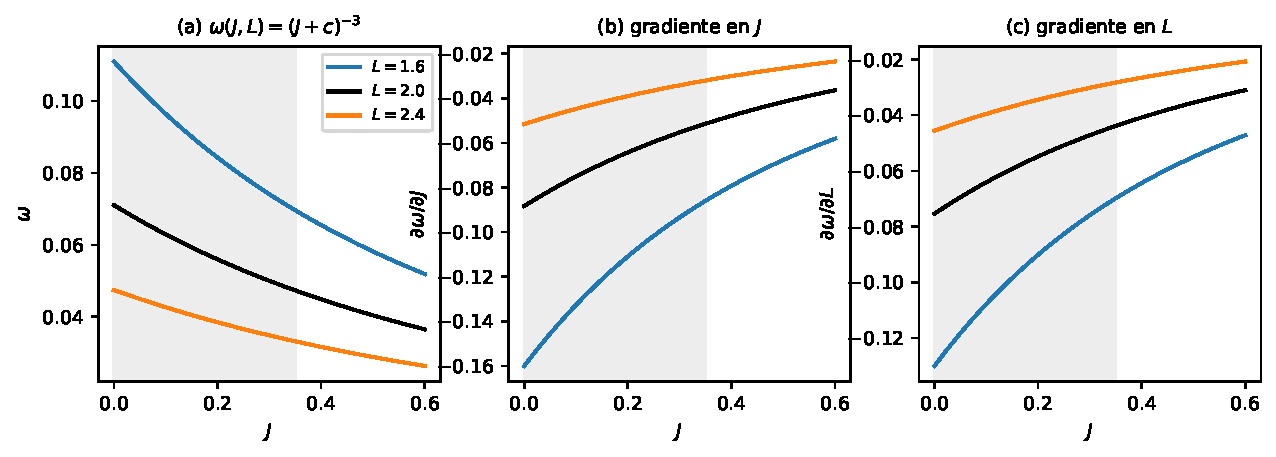
\includegraphics[width=\textwidth]{frecuencias}
  \caption{Frecuencia radial del isócrono y sus dos gradientes, para $L=1.6$, $2$ y
  $2.4$. La franja gris es el soporte en $J$ de las distribuciones de estas notas. En
  $J=0.1$, $L=2$: $\omega=0.0629$, $\partial_J\omega=-0.0751$ y
  $\partial_L\omega=-0.0641$. Una unidad de $L$ cambia la frecuencia el $85\%$ de lo que
  la cambia una unidad de $J$.}
  \label{fig:frecuencias}
\end{figure}

La figura~\ref{fig:frecuencias} muestra lo que importa. En $J=0.1$ y $L=2$ los dos
gradientes valen $-0.0751$ y $-0.0641$: \textbf{una dispersión en $L$ desfasa las órbitas
casi tanto como una dispersión igual en $J$}. Y la banda de frecuencias se ensancha
mucho: sobre $J\in[0,0.35]$, $\omega$ recorre $[0.0473,0.0711]$ con $L=2$, pero
$[0.0696,0.1110]$ con $L=1.6$ y $[0.0332,0.0475]$ con $L=2.4$. Las órbitas de $L$ menor
son más rápidas en todo el soporte.

\subsection{El mapa explícito}
\label{sec:mapa}

Dada $(r,p_r,L)$, la energía da los puntos de retorno,
$r_\pm^2=\big[1+E(2+L^2)\pm\sqrt{1+2E(2+2E+L^2)}\big]/(2E^2)$; con
$s=1+\sqrt{1+r^2}$,
\begin{equation}
  \cos\eta=\frac{s_-+s_+-2s}{s_+-s_-},\qquad Q=\eta-e\sin\eta,
  \label{eq:kepler}
\end{equation}
con una excentricidad efectiva $e(E,L)$ y $\eta\in[0,\pi]$ si $p_r\ge0$. El mapa directo
es explícito; el inverso exige resolver la ecuación de Kepler $Q=\eta-e\sin\eta$ por
Newton. En el código es \texttt{invert\_QJ\_to\_rp} (\texttt{src/utils.f90}), con $L$ por
partícula.

\begin{aviso}
\textsc{detalle numérico: la ida y vuelta.} Se invirtieron 480\,000 puntos
$(Q,J,L)$, con $L=0.05$, $0.6$ y $2.4$ y $J$ hasta 3, y se volvió con el mapa directo:
$Q$ se recupera a $\leq4.6\times10^{-12}$ y $J$ a $\leq6.7\times10^{-15}$, sin ningún NaN.
El error de $Q$ es mayor porque $\arccos$ está mal condicionado cerca de los puntos de
retorno.
\end{aviso}

% ===========================================================================
\section{Phase mixing en dos direcciones}
\label{sec:mixing}

\subsection{Lo que se ve}

La figura~\ref{fig:mezcla} evalúa la solución exacta~\eqref{eq:solucion} para una
distribución concentrada en $Q=0$ en dos cortes: a $L=2$ fijo en el plano $(Q,J)$, y a
$J=0.1$ fijo en el plano $(Q,L)$. En los dos la mancha se inclina y se parte en franjas.
La separación entre franjas del armónico $k$ es
\begin{equation}
  \Delta J=\frac{2\pi}{k|\partial_J\omega|\,t},\qquad
  \Delta L=\frac{2\pi}{k|\partial_L\omega|\,t},
  \label{eq:franja}
\end{equation}
que para $k=1$ vale $\Delta J=0.209$, $\Delta L=0.245$ en $t=400$ y $\Delta J=0.042$,
$\Delta L=0.049$ en $t=2000$.

\begin{figure}[t]
  \centering
  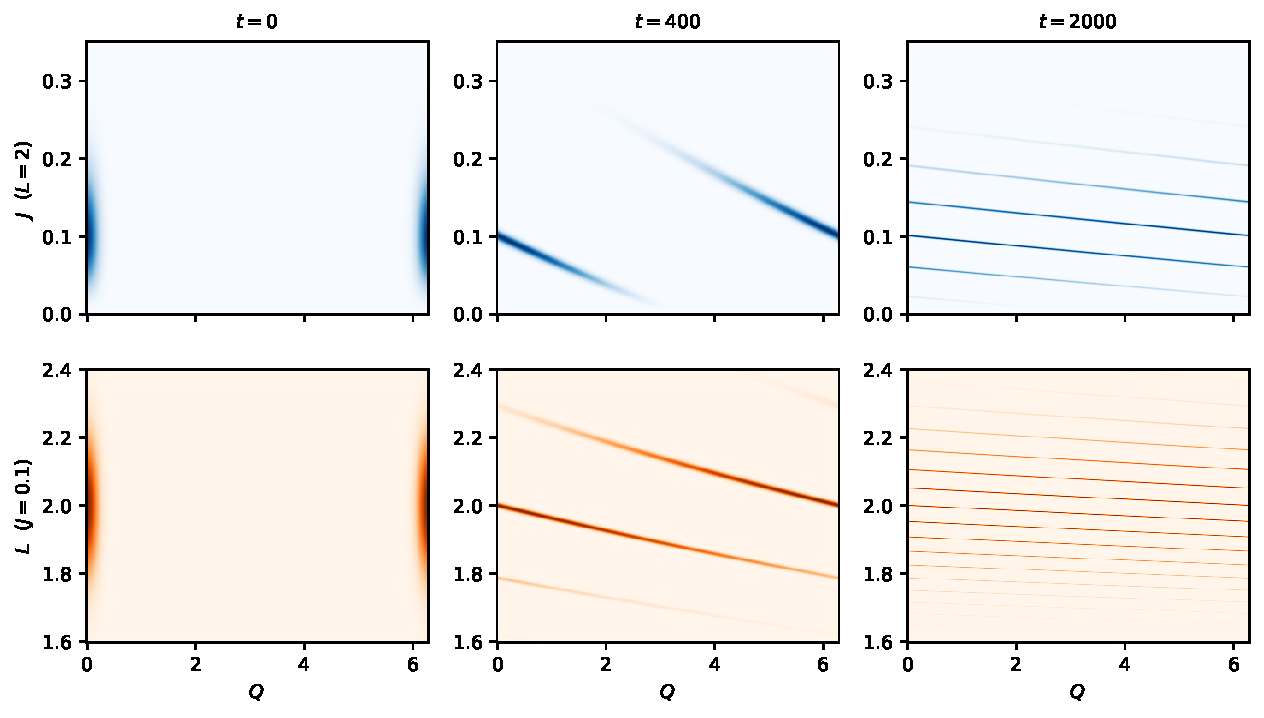
\includegraphics[width=0.95\textwidth]{mezcla}
  \caption{Solución exacta sin autogravedad de
  $F_0=\exp[-\sin^2(Q/2)/0.1^2]\,J^2\ee^{-J^2/0.1^2}\,\ee^{-(L-2)^2/0.2^2}$ en el isócrono.
  \textbf{Arriba}: corte a $L=2$; cada fila de $J$ gira a su frecuencia. \textbf{Abajo}:
  corte a $J=0.1$; cada fila de $L$ también. En $t=2000$ las franjas en $L$ no son
  equiespaciadas porque $\omega$ no es lineal en $L$: el lado de $L$ pequeño gira más rápido
  y se afina antes.}
  \label{fig:mezcla}
\end{figure}

\subsection{El observable}

Proyectamos sobre una función de prueba separable $\Phi_{\rm p}=A(Q)B(J)C(L)$ y nos
quedamos con los armónicos en $Q$:
\begin{equation}
  h_k(t)=8\pi^2\int F\,A(Q)B(J)C(L)\,\ee^{-\ii kQ}\,L\,\dd Q\,\dd J\,\dd L ,
  \label{eq:hk}
\end{equation}
\begin{equation}
  A=\exp\Big[-\frac{\sin^2(Q/2)}{\sigma_Q^2}\Big],\quad
  B=J^2\exp\Big[-\frac{(J-J_t)^2}{\sigma_J^2}\Big],\quad
  C=\exp\Big[-\frac{(L-L_t)^2}{\sigma_{L,t}^2}\Big].
  \label{eq:prueba}
\end{equation}
El código calcula dos funciones de prueba con parámetros propios
(\texttt{j1 sj1 sq1 lt1 slt1} y los mismos con 2) y escribe $h_k$ con su fase.

\subsection{La solución cerrada}

Con $a_k=\frac1{2\pi}\int A\,\ee^{-\ii kQ}\dd Q$ y los coeficientes de la distribución
inicial $F_k(J,L)=\frac1{2\pi}\int F_0\,\ee^{-\ii kQ}\dd Q$, sustituir~\eqref{eq:solucion}
en~\eqref{eq:hk} y normalizar a la masa $a_0$ da
\begin{equation}
  \boxed{\;h_k(t)=a_0\,a_k\,
  \frac{\displaystyle\iint L\,C(L)\,B(J)\,F_k(J,L)\,\ee^{-\ii k\omega(J,L)t}\,\dd J\,\dd L}
       {\displaystyle\iint L\,F_{k=0}(J,L)\,\dd J\,\dd L}\;}
  \label{eq:hkexacto}
\end{equation}
donde $F_{k=0}$ es la distribución inicial promediada en $Q$.
Vale para cualquier $F_0$, separable o no. $h_0$ no oscila: es constante sin
autogravedad. La herramienta \texttt{tools/hk\_exacto.py} evalúa~\eqref{eq:hkexacto}.

\subsection{La envolvente, con dos anchos}

Si el integrando está concentrado alrededor de $(J_0,L_0)$ con segundos momentos
$\mathrm{var}_J$ y $\mathrm{var}_L$, se linealiza
$\omega\simeq\omega_0+\partial_J\omega\,\delta J+\partial_L\omega\,\delta L$ y la
transformada de Fourier de una gaussiana da
\begin{equation}
  \boxed{\;|h_k(t)|\propto\exp\Big[-\frac{k^2t^2}{2}\big(
     (\partial_J\omega)^2\,\mathrm{var}_J+(\partial_L\omega)^2\,\mathrm{var}_L\big)\Big]\;}
  \label{eq:gaussiana}
\end{equation}
Sigue siendo una \textbf{gaussiana en el tiempo}, la firma del phase mixing, pero ahora
con dos contribuciones que se suman en el exponente.

\begin{figure}[t]
  \centering
  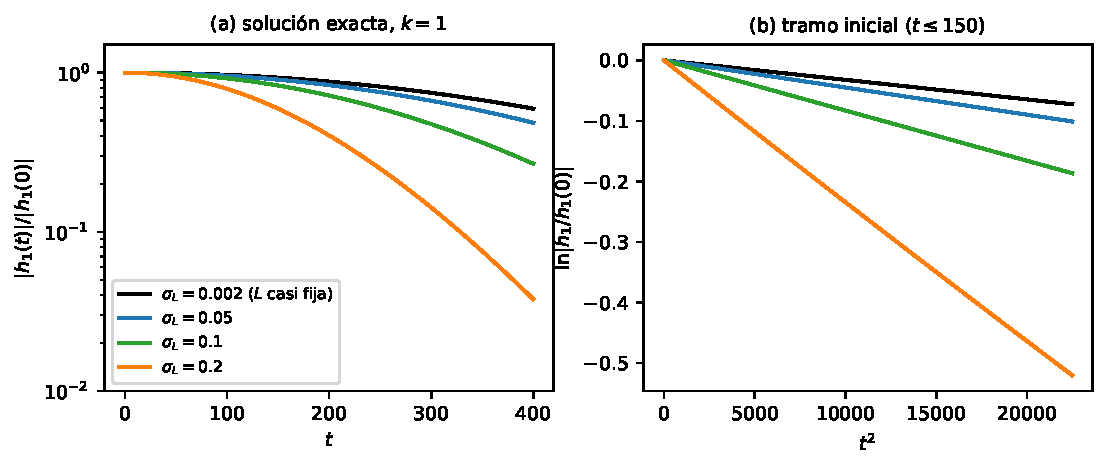
\includegraphics[width=0.95\textwidth]{envolvente}
  \caption{Solución exacta~\eqref{eq:hkexacto} para la distribución gaussiana, con
  función de prueba igual a la distribución, y distintos anchos $\sigma_L$ (soporte
  $[2-4\sigma_L,\,2+4\sigma_L]$). \textbf{(a)} $|h_1|$. \textbf{(b)} $\ln|h_1|$ frente a
  $t^2$ en $t\le150$: rectas, cuya pendiente crece con $\sigma_L$.}
  \label{fig:envolvente}
\end{figure}

La figura~\ref{fig:envolvente} lo comprueba sin aproximaciones. Se ajustó la pendiente de
$\ln|h_1|$ frente a $t^2$ con $L$ casi fijo ($\sigma_L=0.002$): $-3.23\times10^{-6}$. Lo
que la dispersión en $L$ \emph{agrega} a esa pendiente se compara con el término en $L$
de~\eqref{eq:gaussiana}, con $\mathrm{var}_L$ el segundo momento del peso $L\,C_f\,C_t$:

\begin{center}
\begin{tabular}{lccc}
\toprule
$\sigma_L$ & pendiente medida & exceso sobre $L$ fijo & predicción $-\tfrac12(\partial_L\omega)^2\mathrm{var}_L$ \\
\midrule
$0.05$ & $-4.49\times10^{-6}$ & $-1.267\times10^{-6}$ & $-1.283\times10^{-6}$ \\
$0.1$  & $-8.29\times10^{-6}$ & $-5.07\times10^{-6}$  & $-5.13\times10^{-6}$ \\
$0.2$  & $-2.32\times10^{-5}$ & $-2.00\times10^{-5}$  & $-2.05\times10^{-5}$ \\
\bottomrule
\end{tabular}
\end{center}

La predicción lineal acierta al $1$--$2.5\%$; la diferencia crece con $\sigma_L$, lo que es
compatible con que la curvatura de $\omega(L)$, que la linealización ignora, empiece a
pesar. Con $\sigma_L=0.2$, el valor de
las entradas del código, \textbf{la dispersión en $L$ aporta seis veces más a la mezcla
que la dispersión en $J$}: el phase mixing de este sistema lo domina el momento angular.

\subsection{Consecuencia numérica: Nyquist en dos direcciones}

Las franjas~\eqref{eq:franja} se afinan como $1/t$ en $J$ y en $L$. Una rejilla con $N_J$
filas en $J$ y $N_L$ en $L$ las resuelve mientras
\begin{equation}
  N_J\gtrsim\frac{4k\,\Delta\omega_J\,t_{\max}}{2\pi},\qquad
  N_L\gtrsim\frac{4k\,\Delta\omega_L\,t_{\max}}{2\pi},
  \label{eq:nyquist}
\end{equation}
con $\Delta\omega_{J,L}$ el rango de frecuencias que abarca la distribución en cada
dirección. Por debajo, el resultado no es mediocre: es \emph{aliasing}, la recurrencia de
Cheng y Knorr~\cite{chengknorr1976}. La sección~\ref{sec:espiral} la muestra en $L$.

% ===========================================================================
\section{Amortiguamiento de Landau: en qué se diferencia}
\label{sec:landau}

Con autogravedad la perturbación de densidad genera un potencial que actúa sobre las
órbitas. Linealizando alrededor de un equilibrio $F_{\rm eq}(J,L)$, en sus variables
$(Q,J,L)$,
\begin{equation}
  \frac{\partial\,\delta F}{\partial t}+\omega(J,L)\frac{\partial\,\delta F}{\partial Q}
  =\frac{\partial F_{\rm eq}}{\partial J}\,\frac{\partial\,\delta\Phi}{\partial Q}.
  \label{eq:lineal}
\end{equation}
Las partículas resonantes, con $k\,\omega(J,L)=\omega_{\rm modo}$, intercambian energía
con la perturbación y producen un decaimiento exponencial,
$|h_k|\propto\ee^{-\gamma t}$, con $\gamma$ ligado a $\partial_JF_{\rm eq}$ en la
resonancia~\cite{landau1946,binney2008}. Con $L$ fijo la resonancia es un punto $J_{\rm
res}$; \textbf{con distribución en $L$ es una curva} $\omega(J,L)=\omega_{\rm modo}/k$ en
el plano $(J,L)$, y el peso de la resonancia es una integral a lo largo de ella.

\begin{idea}
\textbf{La prueba operativa.} Phase mixing: $\ln|h_k|$ es recta frente a $t^2$.
Amortiguamiento de Landau: recta frente a $t$. Y el control: la misma corrida sin
autogravedad, donde Landau desaparece.
\end{idea}

En las notas con $L$ fijo se midió, en un equilibrio autoconsistente con $a_0=10^{-2}$,
una cola con $\omega=0.05705$ y $\gamma=5.08\times10^{-3}$, independiente de la resolución
y del paso de tiempo y reproducida por la teoría lineal sin partículas. Con distribución
en $L$ \textbf{todavía no se ha medido}; la sección~\ref{sec:preguntas} lo propone.

% ===========================================================================
\section{El método numérico}
\label{sec:metodo}

\subsection{Particle-in-cell}

$F$ se representa con macropartículas $(r,p_r,L,f)$. En cada evaluación de fuerza:
\begin{enumerate}
  \item con autogravedad, cada partícula (una capa de masa $m_j$ en $r_j$) se deposita en
    la malla escalonada $r_i=(i-\tfrac12)\Delta r$ con la función de peso $W_n$
    (B-spline de orden $n=1,2,3$), y la densidad es esa masa entre el volumen que cubre
    el peso,
    \begin{equation}
      \rho_i=\frac{\sum_jm_jW_n\big((r_i-r_j)/\Delta r\big)}{V_i},\qquad
      V_i=4\pi\Delta r\Big(r_i^2+\frac{n+1}{12}\Delta r^2\Big);
    \end{equation}
    cerca del origen se suma también la imagen de cada partícula en $-r_j$, la simetría
    $f(r,p)=f(-r,-p)$;
  \item se integra Poisson, $\dd\Phi/\dd r=M(r)/r^2$, con Runge--Kutta de segundo orden
    desde el centro, y se ajusta la constante para que $\Phi+r\Phi'\to0$ en el borde;
  \item se interpolan potencial y fuerza a cada partícula con el mismo $W_n$ (así no hay
    autofuerza), usando los nodos espejo para $r<\Delta r$ y la solución kepleriana más
    allá del último nodo, y se suman el fondo y el término centrífugo $L^2/r^3$;
  \item se avanzan las partículas.
\end{enumerate}
Referencias clásicas: Birdsall y Langdon~\cite{birdsall2004}, Hockney y
Eastwood~\cite{hockney1988}.

\begin{aviso}
\textsc{detalle numérico: cómo se verificó el acoplamiento.} Con una esfera de densidad
uniforme (radio 5, 2000 capas) y partículas de prueba sin masa, la fuerza sobre las
partículas coincide con $-M(<r)/r^2$ a $6\times10^{-8}$ con $n=2,3$, desde $r=0.01$
hasta fuera de la malla; ese número es la precisión con que las capas representan la
esfera. Con una sola capa, la fuerza es nula adentro, $-0.49\,M/R^2$ sobre la capa (el
límite continuo es $-\tfrac12$) y $-M/r^2$ afuera. Una revisión del código contra estas
ecuaciones encontró y corrigió que la interpolación ignoraba los nodos espejo (la fuerza
salía entre 3.7 y 5 veces la exacta en $r=0.01$), que el volumen $V_i$ era el de otra
función de peso (densidad uniforme sobrestimada en $1+\Delta r^2/12r^2$) y que las
partículas fuera de la malla no sentían la masa; el detalle está en
\texttt{BUGS\_TODO.md}.
\end{aviso}

\subsection{Integradores}

El sistema es hamiltoniano y se integra con métodos simplécticos~\cite{hairer2006}:
salto de rana \emph{kick--drift--kick} (segundo orden) y la composición de cuarto orden
de Yoshida~\cite{yoshida1990}, con pesos $w_1=1/(2-2^{1/3})$ y
$w_0=-2^{1/3}/(2-2^{1/3})$. Algunos subpasos van hacia atrás en el tiempo; eso es lo que
cancela el error de orden bajo. En el código, yoshida4 son tres pares \emph{kick--drift}:
tres fuerzas por paso, y una cuarta solo en los pasos que escriben diagnósticos.

El paso de tiempo es \textbf{fijo} por omisión: un paso que cambia de un paso a otro rompe
el carácter simpléctico. Hay además un integrador \texttt{analytic}, que avanza cada
partícula con~\eqref{eq:solucion} y el mapa inverso: sin autogravedad es exacto para
cualquier $\Delta t$ y sirve de referencia para medir el error de los otros.

\subsection{Cómo se colocan las partículas}
\label{sec:muestreo}

\paragraph{Rejilla en $(r,p_r,L)$} (estados \texttt{gaussian1} y \texttt{aa}): nodos
regulares en el espacio físico con peso $F$ evaluado ahí.

\paragraph{Cuadratura en $(Q,J,L)$} (estado \texttt{aa\_quad}): puntos medios de una
rejilla con $N_J$ celdas en $[J_{\min},J_{\max}]$, $N_Q$ en $[0,2\pi)$ y $N_L$ en
$[L_{\min},L_{\max}]$, llevados a $(r,p_r)$ con el mapa inverso. Como la transformación es
canónica, todos los nodos pesan lo mismo. \textbf{Esto no es muestreo sino una regla de
cuadratura}: en $Q$ es el trapecio periódico, que converge más rápido que cualquier
potencia~\cite{trefethen2014}; en $J$ y $L$ es la regla del punto medio, que converge
como $N^{-2}$ si el integrando no se anula en los bordes y mucho más rápido si se anula.
En el código con $L$ fijo, cualquier desplazamiento aleatorio de los nodos dejó el error
en $N^{-1/2}$; aquí no hay desplazamientos.

\paragraph{Desde un archivo} (estado \texttt{checkpoint}): una línea
``$r\ p_r\ L\ f$'' por partícula. Así entran estados que el código no construye, como un
equilibrio autoconsistente (sección~\ref{sec:equilibrio}), y así se reanuda desde una
instantánea HDF5.

\subsection{\texorpdfstring{El diagnóstico $h_k$}{El diagnóstico hk}}

La suma que aproxima~\eqref{eq:hk} es
\begin{equation}
  h_k\simeq8\pi^2\,\Delta r_c\Delta p_c\Delta L_c\sum_j f_j\,L_j\,B(J_j)\,C(L_j)\,a_k\,
  \ee^{-\ii kQ_j},
\end{equation}
con $(Q_j,J_j)$ del mapa del isócrono. El coeficiente $a_k$ se calcula una sola vez, con
Simpson de 512 intervalos: con $\sigma_Q=0.1$, 20 intervalos daban un error relativo de
$1.2$--$3.2\times10^{-2}$ frente a la forma cerrada $a_k=\ee^{-x}I_k(x)$, $x=1/2\sigma_Q^2$,
y 512 dan $\leq2.2\times10^{-16}$. Las partículas no ligadas ($E\geq0$) no tienen
variables ángulo--acción y se omiten.

\begin{aviso}
\textsc{detalle numérico: reproducibilidad al último bit.} Una suma con
\texttt{REDUCTION} de OpenMP combina las partes de cada hilo en el orden en que los hilos
terminan, que cambia de una corrida a otra: un programa mínimo con la misma suma dio dos
resultados distintos en seis repeticiones. Por eso energía y $h_k$ acumulan por hilo y
suman las partes en orden fijo: dos corridas iguales dan salidas idénticas bit a bit, lo
que permite probar que un cambio del código es neutral comparando archivos.
\end{aviso}

\subsection{Parámetros y reproducibilidad}

El código lee un archivo \texttt{nombre = valor} con reemplazos en la línea de comandos
(\texttt{./VP\_PIC base.par Nt=2000 directory=x}) y escribe en cada corrida
\texttt{params\_usados.par}, la configuración completa, que vuelve a correr la misma
simulación. Todas las corridas de estas notas están en \texttt{reproducir/} (apéndice).

% ===========================================================================
\section{Verificación del código}
\label{sec:verificacion}

\subsection{Contra la solución exacta, separando dos errores}
\label{sec:exacta}

\begin{table}[ht]
\centering
\small
\caption{Corridas de verificación, sin autogravedad, en el isócrono
(\texttt{reproducir/corridas/08\_verificacion}). Comunes: \texttt{state=aa\_quad},
\texttt{a0=1e-3}, $\sigma_J=\sigma_Q=0.1$, $L_0=2$, $\sigma_L=0.2$,
$L\in[1.6,2.4]$, función de prueba 1 igual a la distribución salvo en king.}
\label{tab:verif}
\begin{tabular}{p{0.16\textwidth}p{0.12\textwidth}p{0.28\textwidth}p{0.34\textwidth}}
\toprule
corrida & \texttt{dftype} & rejilla $N_J\times N_Q\times N_L$ & integración \\
\midrule
\texttt{gauss\_y4} & gauss & $200\times40\times16$ & yoshida4, $\Delta t=0.025$, $t\leq200$ \\
\texttt{gauss\_an} & gauss & $200\times40\times16$ & analytic, $\Delta t=1$, $t\leq200$ \\
\texttt{bim\_y4}, \texttt{bim\_an} & bimodal & $200\times40\times16$ & ídem \\
\texttt{spi\_L0\_an} & spiral & $400\times40\times1$, $L\in[1.9995,2.0005]$ & analytic, $t\leq1500$ \\
\texttt{spi\_L16\_an} & spiral & $200\times40\times16$ & analytic, $t\leq1500$ \\
\texttt{king\_y4}, \texttt{king\_an} & king & $100\times40\times16$ & $t\leq100$; prueba: $\sigma_Q=0.5$, $J_t=0.1$, $\sigma_J=0.2$ \\
\bottomrule
\end{tabular}
\end{table}

Con una cuadratura hay dos fuentes de error bien distintas, y conviene medirlas por
separado:
\begin{itemize}
  \item el \textbf{error de la regla}: la suma sobre los nodos no es la integral;
  \item el \textbf{error de la dinámica}: el integrador y el mapa no llevan cada nodo
    exactamente a $Q_0+\omega t$.
\end{itemize}
Por eso \texttt{hk\_exacto.py} calcula dos referencias: la integral
continua~\eqref{eq:hkexacto} (Gauss--Legendre muy fino) y la \emph{suma discreta exacta}
sobre los mismos nodos que usa el código, avanzados con la fórmula cerrada. La diferencia
código$-$discreto es solo dinámica; discreto$-$continuo es solo regla.

\begin{figure}[t]
  \centering
  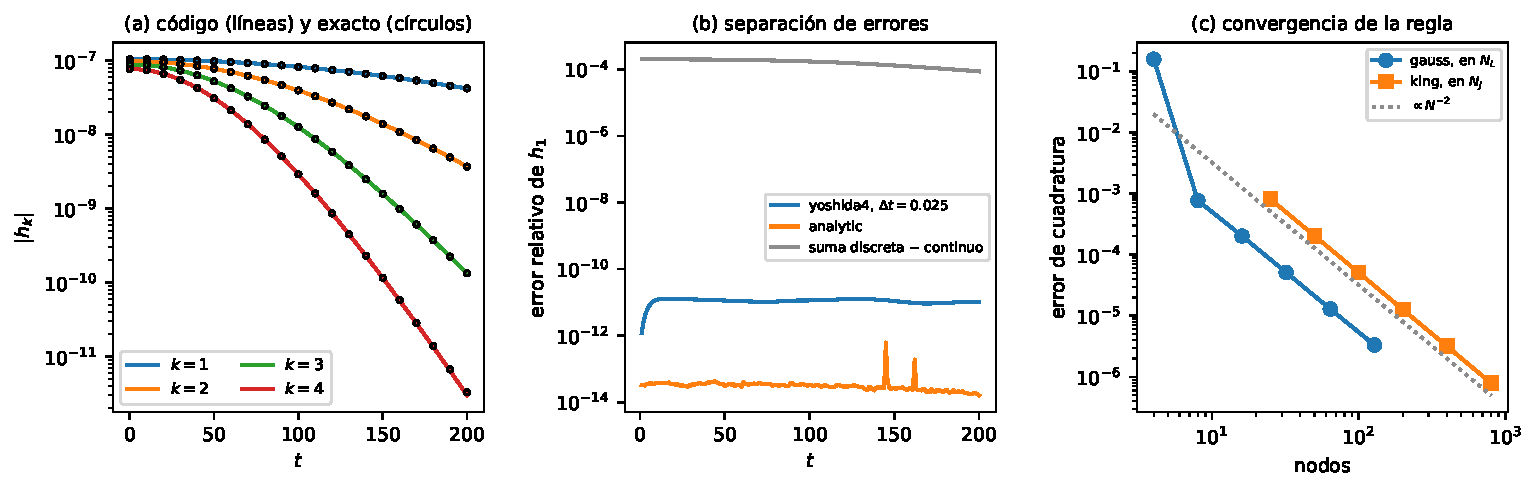
\includegraphics[width=\textwidth]{verificacion}
  \caption{\textbf{(a)} $|h_k|$ del código (líneas) y exacto continuo (círculos), corrida
  \texttt{gauss\_y4}. \textbf{(b)} Error relativo de $h_1$: código menos suma discreta
  exacta con yoshida4 ($1.3\times10^{-11}$) y con analytic ($6.2\times10^{-13}$); en gris,
  suma discreta menos continuo ($2.0\times10^{-4}$), el error de la regla, que domina.
  \textbf{(c)} Error de la regla: gauss al refinar $N_L$ (con $J$ convergido) y king al
  refinar $N_J$ (con $L$ integrado exacto). Ambos $\propto N^{-2}$.}
  \label{fig:verificacion}
\end{figure}

La figura~\ref{fig:verificacion} muestra el resultado. En la corrida con yoshida4 el
código coincide con la suma discreta a $1.3\times10^{-11}$ en $k=1$ ($2.6\times10^{-11}$
en $k=4$), y con \texttt{analytic} a $6.2\times10^{-13}$ ($2.9\times10^{-12}$ en $k=4$), que
es la precisión del mapa. \textbf{Lo que separa al código de la solución exacta es la
regla de cuadratura}, $2.0\times10^{-4}$, y la domina $N_L$: con $J$ ya convergido, el
error baja $4.0\times$ por cada duplicación de $N_L$ ($7.7\times10^{-4}$, $2.0\times10^{-4}$,
$5.1\times10^{-5}$, $1.3\times10^{-5}$, $3.3\times10^{-6}$ para $N_L=8$ a $128$). El
motivo es que $C(L)$ está truncada: en $L=1.6$ y $2.4$ todavía vale $\ee^{-4}$, y el punto
medio con un integrando que no se anula en el borde es de segundo orden. En $J$, en
cambio, el integrando $J^2\ee^{-J^2/\sigma^2}$ se anula en los dos extremos y 200 nodos ya
bastan.

\subsection{Pruebas con otras distribuciones}

Que el acuerdo no dependa de haber elegido una distribución cómoda se prueba con otras
tres, todas multiplicadas por $C(L)$ (\texttt{src/distribution.f90}):

\paragraph{Bimodal, modos prohibidos.}
$F_0=[1+0.8\cos Q+0.3\cos2Q]\,[\ee^{-(J-0.1)^2/0.025^2}+0.7\,\ee^{-(J-0.24)^2/0.035^2}]$.
La parte angular no tiene armónicos por encima de $k=2$, así que $h_3$ y $h_4$ deben ser
exactamente cero en todo tiempo. El código da $|h_3|,|h_4|\leq5.2\times10^{-13}$ de
$\max|h_1|$ con \texttt{analytic} y $\leq7.6\times10^{-12}$ con yoshida4.

\paragraph{King, una esquina.} $F_0=f_{\rm eq}(J,L)(1+0.5\cos Q)$ con
$f_{\rm eq}=\ee^{-E(J,L)/\sigma_E^2}-\ee^{-E(J_t,L)/\sigma_E^2}$ para $J<J_t=0.35$ y cero
después. Código contra suma discreta: $1.3\times10^{-13}$ (\texttt{analytic}) y
$5.2\times10^{-11}$ (yoshida4) en $k=1$; los modos $k\ge2$, prohibidos, quedan en
$\leq2.7\times10^{-11}$. El error de la regla en $N_J$ baja exactamente $4.00\times$ por
duplicación, de $8.1\times10^{-4}$ con $N_J=25$ a $7.9\times10^{-7}$ con $800$
(figura~\ref{fig:verificacion}c).

\paragraph{Espiral.} Se trata en la sección~\ref{sec:espiral}, porque es donde la
dispersión en $L$ cambia cualitativamente el resultado.

\subsection{Energía y fondos}

\begin{table}[ht]
\centering
\small
\caption{Corridas de energía (\texttt{reproducir/corridas/09\_fondos} y
\texttt{10\_energia}). Todas escriben la serie de energía cada \texttt{spatial\_output},
es decir, a intervalos de tiempo iguales.}
\label{tab:energia}
\begin{tabular}{p{0.25\textwidth}p{0.67\textwidth}}
\toprule
grupo & configuración \\
\midrule
fondos & \texttt{state=aa}, \texttt{Nrc=Npc=60}, \texttt{Nlc=1} ($L=2$, nodo en el punto medio de $[1.9995,2.0005]$), \texttt{a0=1e-4}, sin autogravedad, yoshida4, $t=200$; \texttt{BGtype}$\in$\{iso, isotrun, nfw, burkert\}, \texttt{courant}$=0.5,0.25,0.125$ ($\Delta t=0.025$, $0.0125$, $0.00625$) \\
energía & \texttt{a0=1e-3}, autogravedad, yoshida4, $\Delta t=0.025$: \texttt{aa} con $L\in[1.6,2.4]$ y $t=100$; \texttt{gaussian1} con $t=50$; \texttt{aa} con fondo \texttt{sphere} \\
\bottomrule
\end{tabular}
\end{table}

\paragraph{El factor $\tfrac12$.} Con autogravedad la energía conservada es
$\sum_jf_jL_j(\tfrac12p_j^2+\Phi_{\rm fondo}+L_j^2/2r_j^2)+\tfrac12\sum_jf_jL_j\Phi_{\rm
self}(r_j)$: la energía de interacción cuenta cada par una vez. El código sumaba el
potencial propio completo; el cambio de energía reportado era $5.9\times10^{-4}$ (estado
\texttt{aa}) y $4.9\times10^{-4}$ (\texttt{gaussian1}), valores medidos antes de la
corrección. Con el $\tfrac12$, las corridas de la tabla~\ref{tab:energia} dan
$1.9\times10^{-7}$, $2.7\times10^{-7}$ y, con fondo \texttt{sphere}, $1.7\times10^{-7}$. La
trayectoria nunca estuvo afectada: solo la medida.

\paragraph{Fondos analíticos.} Los fondos \texttt{iso}, \texttt{isotrun}, \texttt{nfw} y
\texttt{burkert} no actuaban sobre las partículas (solo llenaban la malla). Corregidos,
sus parejas potencial--fuerza cumplen $F=-\Phi'$ a $10^{-28}$ (comprobado con aritmética
de 30 cifras), y el error máximo de energía converge a cuarto orden:

\begin{center}
\begin{tabular}{lcccc}
\toprule
fondo & $\Delta t=0.025$ & $0.0125$ & $0.00625$ & cocientes \\
\midrule
iso     & $3.13\times10^{-5}$ & $1.92\times10^{-6}$ & $1.20\times10^{-7}$ & $16.3$, $16.0$ \\
isotrun & $7.74\times10^{-7}$ & $4.85\times10^{-8}$ & $3.23\times10^{-9}$ & $16.0$, $15.0$ \\
nfw     & $4.29\times10^{-5}$ & $2.59\times10^{-6}$ & $1.61\times10^{-7}$ & $16.5$, $16.1$ \\
burkert & $7.48\times10^{-6}$ & $4.59\times10^{-7}$ & $2.92\times10^{-8}$ & $16.3$, $15.7$ \\
\bottomrule
\end{tabular}
\end{center}

\begin{aviso}
\textsc{un error de medición que merece quedar escrito.} La primera versión de esta tabla
daba errores de $2\times10^{-8}$ y cocientes sin sentido. La serie de energía se
escribía junto con las instantáneas (\texttt{field\_output}), y al pedir una sola
instantánea final el archivo tenía dos filas: el ``máximo'' se tomaba sobre dos muestras.
Se corrigió en el código (la serie se escribe cada \texttt{spatial\_output}). Antes, en la
bitácora, otra medición con muestreo distinto según $\Delta t$ había dado cocientes entre
10 y 26; con muestreo a intervalos iguales son 15--16.5 en los cuatro fondos.
\end{aviso}

% ===========================================================================
\section{La espiral: desenrollado y dispersión en \texorpdfstring{$L$}{L}}
\label{sec:espiral}

La distribución espiral está enrollada desde el principio:
\begin{equation}
  F_0=\ee^{-(J-0.15)^2/0.04^2}\,\exp\Big[-\frac{\sin^2\big((Q-\beta J)/2\big)}{0.5^2}\Big]\,C(L),
  \qquad\beta=50 .
\end{equation}
El centro angular está en $Q=\beta J$. El phase mixing lo lleva a $Q=\beta
J+\omega(J,L)t$, y con $L$ fijo la inclinación se anula cuando
$\beta+\partial_J\omega\,t=0$:
\begin{equation}
  t^*=-\frac{\beta}{\partial_J\omega(J_0,L_0)}\simeq721 .
\end{equation}
Ahí la distribución se desenrolla y $|h_k|$ \emph{crece} antes de decaer. Es la misma
física que los ecos de plasma: información ``perdida'' por la mezcla que reaparece.

\begin{figure}[t]
  \centering
  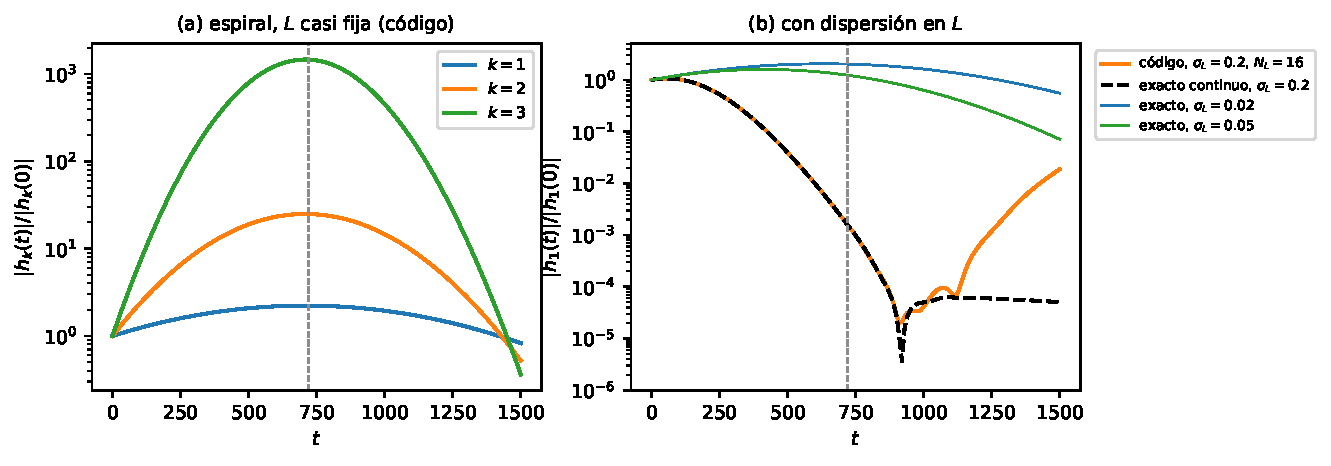
\includegraphics[width=\textwidth]{espiral}
  \caption{\textbf{(a)} Espiral con $L$ casi fijo ($L\in[1.9995,2.0005]$), código con
  \texttt{analytic}: los tres armónicos alcanzan su máximo en $t=710$ (línea: $t^*$
  lineal). \textbf{(b)} Con dispersión en $L$. Negro discontinuo: exacto continuo con
  $\sigma_L=0.2$; el desenrollado desaparece y $|h_1|$ cae a $2.2\times10^{-3}$ en $t=700$.
  Naranja: el código con $N_L=16$, idéntico a la suma discreta, que se separa del continuo
  desde $t\approx1100$ y sube: recurrencia por muestreo en $L$. Azul y verde: exacto
  continuo con $\sigma_L=0.02$ y $0.05$.}
  \label{fig:espiral}
\end{figure}

\paragraph{Con $L$ casi fijo} (figura~\ref{fig:espiral}a), el código reproduce el
desenrollado: $|h_1|$, $|h_2|$ y $|h_3|$ alcanzan su máximo en $t=710$, con $2.2$, $25$ y
$1.5\times10^3$ veces su valor inicial. La diferencia con $t^*=721$ es la curvatura de
$\omega(J)$, que la estimación lineal ignora. Contra la suma discreta, el código coincide a
$\leq5\times10^{-11}$.

\paragraph{Con dispersión en $L$} el resultado cambia por completo. La espiral está
preparada en $J$, pero no en $L$: a $J$ fijo, las filas de distinto $L$ giran a distinta
frecuencia desde $t=0$ sin nada que las vuelva a alinear. Según la solución exacta,
$\max_t|h_1|/|h_1(0)|$ vale $2.05$ (en $t=640$) con $\sigma_L=0.02$, $1.60$ (en $t=410$)
con $\sigma_L=0.05$, y con $\sigma_L=0.2$ ya no hay máximo: $|h_1(700)|/|h_1(0)|=2.2\times10^{-3}$
y $5\times10^{-5}$ desde $t=1000$. \textbf{Una dispersión modesta en momento angular borra
el desenrollado.} La cola que queda en $5\times10^{-5}$ no es gaussiana: la dejan los bordes
del soporte truncado en $L$, que decaen algebraicamente.

\paragraph{Nyquist en $L$.} La corrida del código con $\sigma_L=0.2$ y $N_L=16$ coincide
con la suma discreta a $6\times10^{-14}$ en $k=1$ durante toda la corrida, pero la suma
discreta deja de parecerse a la integral: el cociente código/continuo es $1.2$ en
$t=1100$, $9.7$ en $1200$, $41$ en $1300$ y $143$ en $1400$; en $t=1500$ el código da
$1.9\times10^{-2}$ frente a $5.0\times10^{-5}$. Es la recurrencia de la
condición~\eqref{eq:nyquist}. Dos nodos vecinos en $L$ vuelven a estar en fase cuando su
diferencia de frecuencia acumula $2\pi$; con $\Delta L=0.05$ y $J=0.15$, el primer par en
hacerlo es el de $L$ pequeño, donde $|\partial_L\omega|$ es mayor, en $t\approx1360$. Un
estimado con la frecuencia media, $2\pi N_L/\Delta\omega_L\approx2170$, llega tarde.

\begin{idea}
\textbf{Lo que queda establecido.} (i) El código resuelve correctamente la mezcla en $L$:
coincide con la suma discreta a precisión de máquina. (ii) La dispersión en $L$ suprime
el desenrollado de una estructura preparada en $J$, de manera cuantificable con la
solución exacta. (iii) La rejilla en $L$ tiene su propio tiempo de recurrencia, más corto
que el que sugiere el rango total de frecuencias, y hay que elegir $N_L$ con él.
\end{idea}

% ===========================================================================
\section{Autogravedad: equilibrio \texorpdfstring{$F(J,L)$}{F(J,L)} y el mapa correcto}
\label{sec:equilibrio}

\subsection{El artefacto de coordenadas, otra vez}

El resultado central de las notas con $L$ fijo fue que, con autogravedad, $h_1$ quedaba
en una meseta estática proporcional a la masa que no era un modo sino la huella de
calcular $(Q,J)$ con el mapa del isócrono cuando el potencial es
$\Phi_{\rm iso}+\Phi_{\rm self}$. Con el mapa numérico del potencial real la meseta bajaba
2200 veces. El mismo diagnóstico está en este código, así que se esperaba lo mismo. Para
probarlo de la forma más limpia hace falta un estado que \emph{sea} un equilibrio con
autogravedad.

\subsection{El equilibrio}

\begin{table}[ht]
\centering
\small
\caption{Corridas con autogravedad (\texttt{reproducir/corridas/11\_equilibrio}).
Comunes: \texttt{a0=1e-2}, \texttt{dr=0.05}, \texttt{rmax=25}, yoshida4 con $\Delta
t=0.0125$, $t\leq100$, instantáneas HDF5 cada 5 unidades; rejilla $N_J\times N_Q\times
N_L=200\times20\times8$ (32\,000 partículas), $J\in[0,0.6]$, $L\in[1.6,2.4]$.}
\label{tab:equilibrio}
\begin{tabular}{p{0.14\textwidth}p{0.78\textwidth}}
\toprule
corrida & estado inicial \\
\midrule
\texttt{eq\_e0}  & \texttt{checkpoint}: $F_{\rm eq}=A\,J^2\ee^{-J^2/0.1^2}\ee^{-(L-2)^2/0.2^2}$ con $J$ del potencial total (\texttt{tools/equilibrio\_L.py}) \\
\texttt{eq\_e01} & el mismo, por $1+0.1\cos Q$ \\
\texttt{iso\_aq} & \texttt{aa\_quad}: la misma forma, pero con $(Q,J)$ del isócrono solo; no es equilibrio \\
\midrule
análisis & \texttt{tools/hk\_numerico.py} (mapa numérico, marco instantáneo o \texttt{--equilibrio}), \texttt{tools/delta\_phi.py} \\
\bottomrule
\end{tabular}
\end{table}

Un equilibrio es una función de las acciones del potencial \emph{total}, y el potencial
depende de la distribución. Se itera: potencial propio $\to$ para cada uno de los $N_L$
valores de $L$, tabla $J(E)$ con el mapa numérico $\to$ densidad
\begin{equation}
  4\pi r^2\rho(r)=8\pi^2\sum_kL_k\,\Delta L\int F_{\rm eq}\big(J(E(r,p,L_k)),L_k\big)\,\dd p
\end{equation}
$\to$ Poisson. Cada $L_k$ es un problema de un grado de libertad en el mismo potencial.
Como $\dd r\,\dd p_r=\dd Q\,\dd J$, la masa no depende del potencial y la amplitud $A$
queda fija de entrada.

Con $a_0=10^{-2}$ la iteración converge en seis pasos, con el cambio máximo del
potencial propio bajando de $1.6\times10^{-3}$ a $1.6\times10^{-13}$ (un factor $\sim80$ por
iteración) y la masa exacta a $3.4\times10^{-9}$. Los nodos se colocan en una rejilla de
las $(Q,J,L)$ verdaderas y se invierte el mapa; mapeados de vuelta, se recuperan a
$2.8\times10^{-16}$ en $J$ y $1.7\times10^{-9}$ en $Q$.

\begin{aviso}
\textsc{detalle numérico: el mapa numérico con $L$.} \texttt{tools/aa\_numerico\_L.py}
interpola el potencial propio con un spline cúbico natural (fuera de la tabla, $-M/r$),
localiza la órbita circular de cada $L$ por bisección sobre $\partial_r\Phi_{\rm ef}$,
los puntos de retorno por bisección, y calcula~\eqref{eq:accion} con la sustitución
$r=r_m+r_a\sin\theta$, que cancela la singularidad de los puntos de retorno, y 64 nodos de
Gauss--Legendre. Sin tabla, contra el mapa analítico del isócrono y sobre 14\,556
partículas con $L\in[0.1,3]$: $J$ a $8.9\times10^{-15}$ y $Q$ a $\leq2.7\times10^{-8}$ (el peor caso,
órbitas casi circulares). El inverso usa la tabla $J(E)$ de cada $L$ corregida con
Newton, $\partial E/\partial J=2\pi/T_r$: $J$ a $1.2\times10^{-15}$ y $Q$ a $4.8\times10^{-9}$.
\end{aviso}

\subsection{¿Se queda quieto?}

\begin{figure}[t]
  \centering
  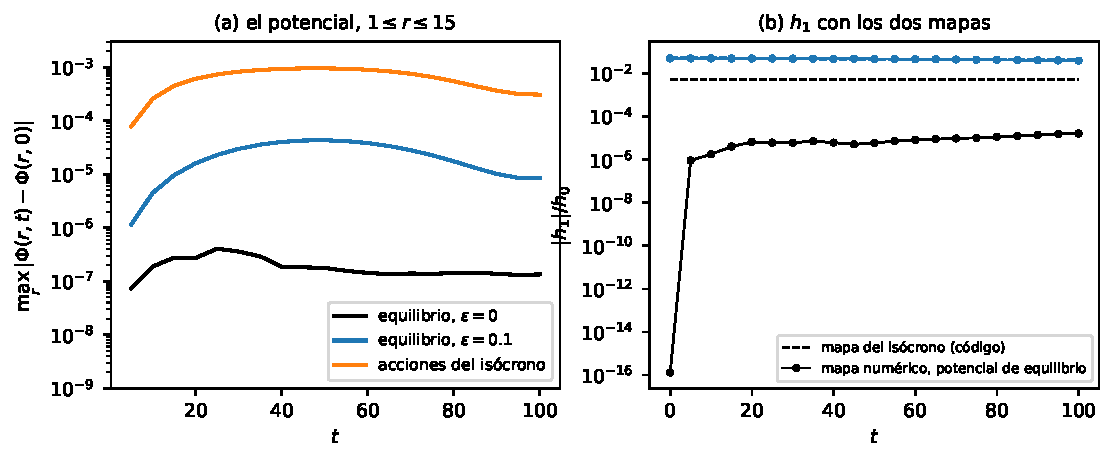
\includegraphics[width=\textwidth]{equilibrio}
  \caption{\textbf{(a)} Cambio máximo del potencial en $1\leq r\leq15$. El equilibrio
  (negro) se mueve $4\times10^{-7}$; con $\varepsilon=0.1$ (azul), $4.3\times10^{-5}$; la misma
  forma en acciones del isócrono (naranja), $9.6\times10^{-4}$. \textbf{(b)} $|h_1|/h_0$
  sobre las mismas partículas con el mapa del isócrono (discontinuo) y con el mapa
  numérico en el potencial de equilibrio (círculos). En el equilibrio la meseta de
  $5\times10^{-3}$ es enteramente artefacto: con el mapa correcto vale $10^{-16}$ en $t=0$.}
  \label{fig:equilibrio}
\end{figure}

En $t=0$ el potencial del código difiere del calculado en Python a lo sumo
$1.4\times10^{-7}$ en $1\leq r\leq15$, frente a $|\Phi_{\rm self}|\leq1.6\times10^{-3}$: es el
desajuste entre el Poisson continuo y el discreto. Durante la corrida
(figura~\ref{fig:equilibrio}a) el potencial del equilibrio se mueve a lo sumo
$4.1\times10^{-7}$, el mismo orden; con la perturbación $\varepsilon=0.1$ se mueve 100
veces más, y con la misma forma de $F$ construida en acciones del isócrono, 2300 veces más.
\textbf{El equilibrio construido es equilibrio del código.}

\subsection{\texorpdfstring{$h_1$ con los dos mapas}{h1 con los dos mapas}}

\begin{center}
\begin{tabular}{lccc}
\toprule
$|h_1|/h_0$ & $t=0$ & $t=50$ & $t=100$ \\
\midrule
equilibrio, mapa del isócrono & $4.958\times10^{-3}$ & $4.952\times10^{-3}$ & $4.971\times10^{-3}$ \\
equilibrio, mapa numérico (potencial de equilibrio) & $1.3\times10^{-16}$ & $6.0\times10^{-6}$ & $1.6\times10^{-5}$ \\
$\varepsilon=0.1$, mapa del isócrono & $5.447\times10^{-2}$ & $4.157\times10^{-2}$ & $4.385\times10^{-2}$ \\
$\varepsilon=0.1$, mapa numérico (potencial de equilibrio) & $4.950\times10^{-2}$ & $4.659\times10^{-2}$ & $3.889\times10^{-2}$ \\
\bottomrule
\end{tabular}
\end{center}

Con el mapa del isócrono, el equilibrio muestra una meseta de $4.96\times10^{-3}\,h_0$
constante: la versión con distribución en $L$ del artefacto. Con el mapa del potencial
real vale $10^{-16}$ en $t=0$ y crece hasta $1.6\times10^{-5}$ en $t=100$, al ritmo del
desajuste del Poisson discreto. Con la perturbación, el valor inicial esperado es
exactamente $(a_1/a_0)\,\varepsilon/2=0.04950$; el mapa numérico da $0.04950$ y el del
isócrono $0.0545$, un $10\%$ de error sobre las mismas partículas.

\begin{aviso}
\textsc{¿respecto de qué potencial?} La primera versión de este análisis usó el potencial
\emph{instantáneo} de cada instantánea y dio $0.04936$ en $t=0$, un $0.3\%$ por debajo de lo
esperado. No era un error del mapa: la perturbación $\varepsilon\cos Q$ ya cambia la
densidad radial en $t=0$, y el potencial propio instantáneo difiere del de equilibrio en
$2.3\times10^{-5}$, lo que desplaza las acciones hasta $6\times10^{-4}$. Para una
perturbación, el marco natural es el potencial fijo del equilibrio
(\texttt{hk\_numerico.py --equilibrio}); para el equilibrio mismo los dos marcos casi
coinciden ($2.5\times10^{-7}$ en $t=0$ con el instantáneo).
\end{aviso}

Hasta $t=100$ la respuesta con $\varepsilon=0.1$ decae de $0.0495$ a $0.0389$. Con corridas
de ese largo no se puede decir nada sobre amortiguamiento de Landau: con $L$ fijo la cola
colectiva apareció después de $t\approx1000$.

% ===========================================================================
\section{Cuánto cuesta}
\label{sec:costo}

Con 128\,000 partículas \texttt{aa\_quad}, cuatro hilos, un portátil con un Intel i7-4710HQ,
las mejoras de rendimiento (todas idénticas bit a bit en las salidas) llevaron 300 pasos
con autogravedad de $25.0$ a $11.6$~s y 1000 pasos sin autogravedad de $10.4$ a $4.3$~s
(promedios de corridas intercaladas A--B--B--A). Con autogravedad eso es
$\approx39$~ms por paso: escalando con el número de partículas, un equilibrio de $10^5$
partículas hasta $t=3000$ con $\Delta t=0.025$ ($1.2\times10^5$ pasos) tarda del orden de una
hora. Lo caro es el depósito de densidad y la interpolación: antes de optimizar eran el
$80\%$ del tiempo con autogravedad.

Lo que decide cuántas partículas hacen falta no es $N$ sino su reparto:
$N_Q\sim20$--$40$ (el trapecio periódico converge enseguida) y $N_J$, $N_L$
según~\eqref{eq:nyquist} para el $t_{\max}$ que se quiera. Con $\sigma_L=0.2$ la
condición en $L$ es la más exigente: para $k=1$ y $t_{\max}=2000$, la recurrencia del par de
nodos más rápido exige $\Delta L\lesssim2\pi/(k|\partial_L\omega|_{\max}t_{\max})$; con
$|\partial_L\omega|_{\max}=0.130$ (en $J=0$, $L=1.6$) eso es $\Delta L\lesssim0.024$, es decir
$N_L\gtrsim33$ en $[1.6,2.4]$, y proporcionalmente más para $k>1$. Es un criterio de orden
de magnitud: en la sección~\ref{sec:espiral} la recurrencia empezó algo antes de lo que
predice.

% ===========================================================================
\section{Lecciones de método}

\begin{enumerate}
  \item \textbf{Separar los errores.} Comparar contra la suma discreta exacta y no solo
    contra la integral dice cuál de los dos errores domina. Aquí el integrador era
    $10^{-11}$ y la regla $10^{-4}$: refinar $\Delta t$ no habría servido de nada.
  \item \textbf{Un número demasiado bueno también es sospechoso.} El error de energía de
    $2\times10^{-8}$ de los fondos no era precisión: era un máximo sobre dos muestras.
  \item \textbf{Preguntar qué calcula exactamente la línea que produce un número.} La
    meseta de $h_1$ es el mapa equivocado; el $0.3\%$ del caso perturbado, el marco
    equivocado; el error de energía de $5\times10^{-4}$, un $\tfrac12$ ausente. Ninguno era
    dinámica.
  \item \textbf{Hacer el código reproducible bit a bit}, incluidas las sumas en paralelo.
    Así cada cambio que no debía alterar resultados se probó comparando archivos, y los que
    sí los alteraban se midieron.
  \item \textbf{Leer los diagnósticos que nadie usa.} La densidad media de una cáscara
    que escribía el código crecía con $N_L$ (23 y 95 veces la real con $N_L=4$ y $16$): le
    faltaban el peso $L$ y el volumen de celda.
\end{enumerate}

% ===========================================================================
\section{Relación con la literatura}
\label{sec:literatura}

El phase mixing en un potencial central externo con partículas de momento angular fijo lo
estudiaron Rioseco y Sarbach~\cite{rioseco2020}. Chaturvedi y Luk~\cite{chaturvedi2024}
demuestran phase mixing lineal y no lineal para Vlasov--Poisson con un Kepler externo en
simetría esférica, con variables ángulo--acción definidas a partir del potencial
autoconsistente: es la versión rigurosa de lo que aquí se construye numéricamente. La
cuadratura en ángulo--acción es el \emph{quiet start} de Sellwood~\cite{sellwood1997}, y
el umbral de resolución, la recurrencia de Cheng y Knorr~\cite{chengknorr1976}. Que las
acciones calculadas en un potencial aproximado oscilen es conocido~\cite{sanders2016,burger2021}.

Sobre modos y amortiguamiento en sistemas esféricos: Weinberg~\cite{weinberg1994} mostró
modos débilmente amortiguados; Fouvry y Prunet~\cite{fouvry2022} desarrollan el método
matricial con continuación analítica y encuentran un modo $\ell=1$ débilmente amortiguado
en el isócrono; Polyachenko, Shukhman y Borodina~\cite{polyachenko2021} distinguen modos
genuinos de ondas amortiguadas por Landau; Ramming y Rein~\cite{ramming2018} y
Straub~\cite{straub2024} estudian numéricamente perturbaciones $\ell=0$ alrededor de
equilibrios esféricos. Los ecos, la reaparición de una perturbación mezclada, son un
fenómeno clásico en plasmas y en galaxias.

\begin{aviso}
\textsc{cautela.} Esta sección resume lo que se sabe de esos trabajos por sus resúmenes y
por la búsqueda hecha para las notas con $L$ fijo. En particular no se ha verificado si
la supresión del desenrollado por dispersión en $L$ (sección~\ref{sec:espiral}) o la
dependencia de $\gamma$ con $\sigma_L$ ya están descritas: antes de afirmar novedad hay
que leer completos~\cite{fouvry2022,straub2024,chaturvedi2024} y buscar específicamente
ecos en sistemas esféricos con distribución en momento angular.
\end{aviso}

% ===========================================================================
\section{Preguntas para un artículo}
\label{sec:preguntas}

Lo que sigue son preguntas concretas que este código, en su estado actual, permite atacar,
ordenadas de la más cercana a la más ambiciosa. Para cada una: qué se sabe ya, qué haría
falta medir y qué la haría publicable.

\begin{pregunta}
\textbf{P1. ¿Cómo suprime la dispersión en momento angular la reversibilidad del phase
mixing?}

\emph{Qué hay.} La solución exacta y el código muestran que el desenrollado de una espiral
preparada en $J$ ($2.2\times$ en $t=710$ con $L$ fijo) baja a $2.05\times$ con
$\sigma_L=0.02$, $1.6\times$ con $0.05$ y desaparece con $0.2$ (sección~\ref{sec:espiral}).
La envolvente gaussiana suma las contribuciones en $J$ y $L$ al $1$--$2.5\%$
(sección~\ref{sec:mixing}).

\emph{Qué medir.} La amplitud del máximo como función de $\sigma_L$ y de la forma de $C(L)$
(gaussiana, truncada, compacta), y una ley cerrada: con la linealización, la amplitud del
eco debería caer como $\exp[-\tfrac12k^2(\partial_L\omega)^2\mathrm{var}_L\,t^{*2}]$. Luego
ecos propiamente dichos: una segunda perturbación en $t_1$ y la respuesta en $t_2$, con y
sin dispersión en $L$, y con autogravedad.

\emph{Por qué importa.} Las estructuras de phase mixing que persisten o reaparecen se usan
como huella de perturbaciones pasadas; si una dispersión realista en momento angular las
borra, cambia qué se puede inferir de ellas. Es barato: casi todo se hace con \texttt{analytic} y la solución exacta.
\end{pregunta}

\begin{pregunta}
\textbf{P2. Amortiguamiento de Landau en un equilibrio $F(J,L)$: ¿cómo dependen
$\omega$ y $\gamma$ de $\sigma_L$?}

\emph{Qué hay.} Con $L$ fijo: $\omega=0.05705$, $\gamma=5.08\times10^{-3}$, validados con
resolución, $\Delta t$ y teoría lineal. Con $L$ distribuida: el equilibrio
autoconsistente, verificado como equilibrio del código ($\delta\Phi\sim4\times10^{-7}$), la
perturbación y el mapa numérico en el marco correcto (sección~\ref{sec:equilibrio}).

\emph{Qué medir.} Corridas hasta $t\approx3000$ con $\varepsilon=0$ y $0.1$ (restando la
primera), $a_0=10^{-2}$ y $\sigma_L\to0,\ 0.05,\ 0.1,\ 0.2$; ajuste de la cola con
\emph{matrix pencil}; controles de $N_J$, $N_L$ y $\Delta t$. Con $L$ distribuida la
resonancia es una curva en $(J,L)$, así que $\gamma$ debería depender de $\sigma_L$; si
$\sigma_L\to0$ reproduce el valor de $L$ fijo, eso además valida el montaje.

\emph{Costo.} Del orden de una hora y media por corrida con $10^5$ partículas
(sección~\ref{sec:costo}); unas diez corridas.
\end{pregunta}

\begin{pregunta}
\textbf{P3. Teoría lineal con distribución en $L$.}

\emph{Qué hay.} El solver lineal sin partículas de las notas con $L$ fijo (transporte
exacto en $Q$, función de Green de capas esféricas) reprodujo la simulación a $0.1\%$
hasta $t=800$.

\emph{Qué hacer.} Extenderlo a $\delta F(Q,J,L)$: una rejilla más, y la función de Green
sigue siendo la misma porque la perturbación es esférica. Comparar con P2. Si además se
hace la continuación analítica de la relación de dispersión~\cite{fouvry2022}, se puede
decidir si la cola es un polo, un modo de Landau en sentido estricto.
\end{pregunta}

\begin{pregunta}
\textbf{P4. ¿Cuándo basta el mapa del isócrono?}

\emph{Qué hay.} La meseta artificial vale $4.96\times10^{-3}h_0$ con $a_0=10^{-2}$ y
$\sigma_L=0.2$. Con $L$ fijo y la misma masa se midió $1.2\times10^{-2}h_0$, pero en otro
montaje (una distribución que no era equilibrio con autogravedad), así que los dos números
no son comparables todavía. El error en una perturbación es del $10\%$ al comienzo.

\emph{Qué medir.} La meseta frente a $a_0$ y $\sigma_L$ y un criterio práctico ``el mapa
analítico sirve para señales mayores que $\alpha\,a_0\,h_0$''. Es un resultado de métodos
útil para cualquiera que use acciones analíticas en simulaciones con autogravedad, y sale
casi gratis de las corridas de P2.
\end{pregunta}

\begin{pregunta}
\textbf{P5. El piso de ruido de discreción con autogravedad y distribución en $L$.}

\emph{Qué hay.} Con $L$ fijo, después de la mezcla quedaba una componente de $h_1$ que
dependía de la resolución, $\sim10^{-4}h_0$, y crecía como $t^{1.9}$ con $a_0=10^{-2}$. En el
equilibrio de estas notas, el mapa numérico da $|h_1|/h_0$ de $10^{-16}$ en $t=0$ a
$1.6\times10^{-5}$ en $t=100$.

\emph{Qué medir.} Ese crecimiento frente a $N_J$, $N_Q$, $N_L$ y $\Delta r$, para saber
hasta qué $t$ y qué nivel de señal son creíbles las mediciones de P2. Es la condición para
que P2 sea publicable, más que una pregunta en sí.
\end{pregunta}

\begin{pregunta}
\textbf{P6. Régimen no lineal.}

Con $a_0\gtrsim10^{-2}$ el efecto colectivo deja de ser una corrección y puede dominar;
con perturbaciones grandes se llega a la relajación violenta~\cite{lyndenbell1967}. Con la
dispersión en $L$ hay además acoplamiento entre filas de distinto $L$ a través del
potencial común. Es la pregunta más interesante y la menos preparada: requiere primero
P2, P3 y P5.
\end{pregunta}

\paragraph{Propuesta de artículo.} P1 y P4 son autocontenidas y casi listas: la solución
exacta, el código verificado y las herramientas existen. P2 con los controles de P5, y P3
como validación independiente, forman un segundo artículo más fuerte: la primera medición
de amortiguamiento de Landau $\ell=0$ en función de la dispersión en momento angular, con
teoría lineal al lado. Las limitaciones que hay que declarar desde ya: un solo potencial de
fondo (isócrono), perturbaciones esféricas, y el mapa ángulo--acción verdadero solo en
postprocesamiento (el diagnóstico en línea del código sigue usando el del isócrono).

% ===========================================================================
\appendix
\section{Cómo reproducir estas notas}
\label{sec:reproducir}

Desde la raíz del repositorio (rama \texttt{mejoras/portar}), con Python~3,
\texttt{numpy}, \texttt{h5py} y \texttt{matplotlib}:

\begin{verbatim}
make                                   # exe/VP_PIC
reproducir/correr.sh 08_verificacion   # 1.3 min
reproducir/correr.sh 09_fondos         # segundos
reproducir/correr.sh 10_energia        # segundos
reproducir/correr.sh 11_equilibrio     # 5 min, incluye tools/equilibrio_L.py
reproducir/analisis.sh                 # h_k exacto, mapa numérico, delta Phi
python3 reproducir/figuras/generar_figuras.py
cd docs/introduccion && latexmk -pdf vlasov_L_intro.tex
\end{verbatim}

Tiempos medidos con cuatro hilos. Las corridas nunca se lanzan en paralelo.
\texttt{generar\_figuras.py} imprime, para cada figura, las cifras que cita el texto; las
figuras \texttt{frecuencias}, \texttt{mezcla} y \texttt{envolvente}, y la convergencia de la
figura~\ref{fig:verificacion}c, se calculan en Python sin simular. Las cifras de energía
antes de corregir el $\tfrac12$, de rendimiento y de las pruebas de neutralidad de los
cambios están registradas, con su verificación, en \texttt{BUGS\_TODO.md}.

\begin{thebibliography}{99}

\bibitem{arnold1989}
V.~I.~Arnold, \emph{Mathematical Methods of Classical Mechanics}, 2\textsuperscript{a}
ed., Springer, 1989.

\bibitem{binney2008}
J.~Binney y S.~Tremaine, \emph{Galactic Dynamics}, 2\textsuperscript{a} ed., Princeton
University Press, 2008.

\bibitem{birdsall2004}
C.~K.~Birdsall y A.~B.~Langdon, \emph{Plasma Physics via Computer Simulation}, Taylor \&
Francis, 2004.

\bibitem{burger2021}
J.~D.~Burger, J.~Peñarrubia y J.~Zavala, \emph{Conservation of radial actions in
time-dependent spherical potentials}, MNRAS (2021), arXiv:2012.00737.

\bibitem{chaturvedi2024}
S.~Chaturvedi y J.~Luk, \emph{Linear and nonlinear phase mixing for the gravitational
Vlasov--Poisson system under an external Kepler potential}, Arch. Ration. Mech. Anal.
(2026), arXiv:2409.14626.

\bibitem{chengknorr1976}
C.~Z.~Cheng y G.~Knorr, \emph{The integration of the Vlasov equation in configuration
space}, J. Comput. Phys. \textbf{22} (1976) 330.

\bibitem{fouvry2022}
J.-B.~Fouvry y S.~Prunet, \emph{Linear response theory and damped modes of stellar
clusters}, MNRAS \textbf{509} (2022) 2443, arXiv:2105.01371.

\bibitem{goldstein2002}
H.~Goldstein, C.~Poole y J.~Safko, \emph{Classical Mechanics}, 3\textsuperscript{a} ed.,
Addison-Wesley, 2002.

\bibitem{hairer2006}
E.~Hairer, C.~Lubich y G.~Wanner, \emph{Geometric Numerical Integration},
2\textsuperscript{a} ed., Springer, 2006.

\bibitem{henon1959}
M.~Hénon, \emph{L'amas isochrone I}, Annales d'Astrophysique \textbf{22} (1959) 126.

\bibitem{hockney1988}
R.~W.~Hockney y J.~W.~Eastwood, \emph{Computer Simulation Using Particles}, Adam Hilger,
1988.

\bibitem{landau1946}
L.~D.~Landau, \emph{On the vibrations of the electronic plasma}, J. Phys. USSR \textbf{10}
(1946) 25.

\bibitem{landau1976}
L.~D.~Landau y E.~M.~Lifshitz, \emph{Mechanics}, 3\textsuperscript{a} ed.,
Butterworth-Heinemann, 1976.

\bibitem{lyndenbell1967}
D.~Lynden-Bell, \emph{Statistical mechanics of violent relaxation in stellar systems},
MNRAS \textbf{136} (1967) 101.

\bibitem{polyachenko2021}
E.~V.~Polyachenko, I.~G.~Shukhman y O.~I.~Borodina, \emph{Damped perturbations in stellar
systems: genuine modes and Landau-damped waves}, MNRAS \textbf{503} (2021) 660,
arXiv:2101.08287.

\bibitem{ramming2018}
T.~Ramming y G.~Rein, \emph{Oscillating solutions of the Vlasov--Poisson system: a
numerical investigation}, Physica D \textbf{365} (2018) 72, arXiv:1602.07989.

\bibitem{rioseco2020}
P.~Rioseco y O.~Sarbach, \emph{Phase space mixing in an external gravitational central
potential}, Class. Quantum Grav. (2020), arXiv:2005.05988.

\bibitem{sanders2016}
J.~L.~Sanders y J.~Binney, \emph{A review of action estimation methods for galactic
dynamics}, MNRAS \textbf{457} (2016) 2107, arXiv:1511.08213.

\bibitem{sellwood1997}
J.~A.~Sellwood, \emph{Galaxy dynamics by N-body simulation}, en \emph{Computational
Astrophysics}, ASP Conf. Ser. (1997), arXiv:astro-ph/9612087.

\bibitem{straub2024}
C.~Straub, \emph{Numerical experiments on stationary, oscillating, and damped spherical
galaxy models}, Physica D \textbf{470} (2024) 134351, arXiv:2405.01235.

\bibitem{trefethen2014}
L.~N.~Trefethen y J.~A.~C.~Weideman, \emph{The exponentially convergent trapezoidal
rule}, SIAM Review \textbf{56} (2014) 385.

\bibitem{weinberg1994}
M.~D.~Weinberg, \emph{Weakly damped modes in star clusters and galaxies}, ApJ
\textbf{421} (1994) 481.

\bibitem{yoshida1990}
H.~Yoshida, \emph{Construction of higher order symplectic integrators}, Phys. Lett. A
\textbf{150} (1990) 262.

\end{thebibliography}

\end{document}
